\subsection{Problems in two space dimensions}
The formulation developed in the previous section differs from those of \textsc{Bleich} \cite{Bleich}, \textsc{Clifton} \cite{Clifton}, and hence from these of \textsc{Ting} and \textsc{Nan} \cite{Ting68} and \textsc{Ting} \cite{Ting69}, in that equation  \eqref{eq:quasilinear_normal} is based on the elastoplastic stiffnesses rather than softnesses.
As a consequence, it will be seen in what follows that the equations can be easily specialized to plane strain and plane stress cases.

We now focus on the solid domain $x_1 \times x_2 \times x_3 \in [0,\infty[ \times [-h,h] \times [-e,e]$ in a Cartesian coordinate system, where $e$ and $h$ are arbitrary lengths.
%The solid is subject in the plane $x_1=0$ to a traction force $\vect{T}^1$ restricted to the $(\vect{e}_1,\vect{e}_2)$ plane, that is $T_3=0$.
It is assumed that all quantities depend solely on $x_1$ and $x_2$ except the velocity component $v_3$ that may depend on $x_3$.
In particular, this is the case for $e \ll h$.

The solid is under plane strain conditions, that is $\tens{\eps}\cdot\vect{e}_3=\vect{0}$, if the velocity $\vect{v}$ does not depend on $x_3$ and if $v_3$ vanishes.
Thus, combining the additive partition of the infinitesimal strain tensor: $\tens{\eps}=\tens{\eps}^e+\tens{\eps}^p$, with the elastic law \eqref{eq:elastic_inverse} and the kinematic condition $\eps_{33}=0$, one gets:
\begin{equation}
  \label{eq:plane_strain_stress33}
  \sigma_{33}=\nu\(\sigma_{11}+\sigma_{22}\) - E\eps^p_{33}
\end{equation}
Hence, the quasi-linear form \eqref{eq:quasilinear_normal} reduces for plane strain problems to a system of dimension $5$ with unknowns $v_1,v_2, \sigma_{11},\sigma_{12}$, and $\sigma_{22}$.


Alternatively, a plane stress state ($\tens{\sigma}\cdot\vect{e}_3=\vect{0}$) is assumed if the planes $x_3=\pm h$ are traction free and $e\ll h$.
As a result, the stress component $\sigma_{33}$ can be removed from the system \eqref{eq:quasilinear_normal}.
Nevertheless, the tangent modulus must account for the vanishing out-of-plane stress component.
Specialization of equation \eqref{eq:elastoplastic_tangent} to $\sigma_{33}$ yields:
\begin{equation*}
  \dot{\sigma}_{33}=C^{ep}_{33ij} \dot{\eps}_{ij} =0
\end{equation*}
from which one writes:
\begin{equation*}
  C^{ep}_{3333} \dot{\eps}_{33} = - C^{ep}_{33ij}\dot{\eps}_{ij} \quad i,j=\{1,2\}
\end{equation*}
Hence, the constitutive equations are rewritten by means of a two-dimensional tangent modulus $\widetilde{\Cbb}^{ep}$:
\begin{equation}
  \label{eq:CP_constitutive}
  \dot{\sigma}_{ij}=C^{ep}_{ijkl} \dot{\eps}_{kl} - \frac{C^{ep}_{ij33}C^{ep}_{33kl}}{C^{ep}_{3333}}\dot{\eps}_{kl}= \widetilde{C}^{ep}_{ijkl} \dot{\eps}_{kl}\qquad i,j,k,l=\{1,2\} 
\end{equation}
The characteristic structure of the problem is then given by the associated acoustic tensor $\tens{\widetilde{A}}^{ep}=\vect{n}\cdot\widetilde{\Cbb}^{ep}\cdot \vect{n}$.

The removal of $\sigma_{33}$ from system \eqref{eq:quasilinear_normal} for both plane strains and plane stresses allows solving the problem in a two-dimensional setting.
Then, generically denoting the acoustic tensor by $\tens{A}$, the characteristic structures are given by the eigenvalues:
\begin{subequations}
  \begin{alignat}{1}
    \label{eq:eigenAcc1}
    &\omega_1 = \frac{1}{2}\(A_{11}+A_{22} + \sqrt{(A_{11}-A_{22})^2+{4A_{12}}^2}\) \\
    \label{eq:eigenAcc2}
    &\omega_2 = \frac{1}{2}\(A_{11}+A_{22} - \sqrt{(A_{11}-A_{22})^2+{4A_{12}}^2}\)     
  \end{alignat}
\end{subequations}
and the associated eigenvectors:
\begin{equation}
  \label{eq:eigenvectAcc}
   \vect{l}^1=[ A_{22}-  \omega_1 \:,\: -A_{12}] \qquad ;\qquad  \vect{l}^2=[ -A_{12} \:,\:A_{11}- \omega_2 ]
\end{equation}
From equation \eqref{eq:left_eigenfields}, we see that two families of waves with celerities $c_f=\pm \sqrt{\omega_1/\rho}$ and $c_s = \pm \sqrt{\omega_2/\rho}$ may travel in the domain.
These waves are respectively referred to as fast and slow waves.
Note that subtracting equations \eqref{eq:eigenAcc1} and \eqref{eq:eigenAcc2} leads to:
\begin{equation}
  \label{eq:diff_celerities}
  \rho c_f^2 - \rho c_s^2 = \sqrt{(A_{11}-A_{22})^2+{4A_{12}}^2} \geq 0
\end{equation}
Hence, the characteristic speed associated with fast waves is always greater than or equal to that of slow waves.

The four left eigenfields of the Jacobian matrix thus read:
\begin{subequations}
  \begin{alignat}{1}
    \label{eq:Jac_eigenfield_fast}
    &\left\lbrace \pm c_f ; \quad \Lcb^{c_f^\pm}=\[\: \pm \rho c_f \vect{l}^1 , -\vect{l}^1\otimes \vect{n} \:\]  \right\rbrace \\
  \label{eq:Jac_eigenfield_slow}
    &\left\lbrace \pm c_s ; \quad \Lcb^{c_s^\pm}=\[\: \pm \rho c_s \vect{l}^2 , -\vect{l}^2\otimes \vect{n} \:\]  \right\rbrace
  \end{alignat}
\end{subequations}
where $\Lcb^{c_f^+}$ and $\Lcb^{c_f^-}$ are associated with the right-going and left-going fast waves respectively.
The same goes for $\Lcb^{c_s^+}$ and $\Lcb^{c_s^-}$.
Furthermore, one stationary wave associated with the zero eigenvalue of the Jacobian matrix, and whose left eigenvector satisfies equation \eqref{eq:null_eigen}, has to be added:
\begin{equation}
  \label{eq:null_left_eigen}
  {\Lcb^0}^T = \matrice{v_1^0 \\[5.pt] v_2^0 \\[5.pt] \sigma_{11}^0 \\[5.pt] \sigma^0_{22} \\[5.pt] \sigma^0_{12} }= \matrice{0 \\[5.pt] 0 \\[5.pt] \(C_{121i}C_{222j}-C_{221i}C_{122j}\)n_in_j \\[5.pt] \(C_{111i}C_{122j}-C_{112i}C_{121j}\)n_in_j \\[5.pt] \(C_{112i}C_{221j}-C_{111i}C_{222j}\)\frac{n_in_j}{2}} = \matrice{0 \\ 0 \\ \alpha_{11} \\ \alpha_{22} \\ \alpha_{12} }
\end{equation}
with $\Cbb=\Cbb^{ep}$ for plain strain and $\Cbb=\widetilde{\Cbb}^{ep}$ for plane stress.
%In particular, $\Cbb$ reduces to the elastic stiffness tensor when no plastic flow occurs so that the characteristic structure involves the speeds of elastic pressure waves $c_1$ and shear waves $c_2$. 

It has been seen in section \ref{sec:SVK_solution} that the solution of non-linear problems may contain shock and/or simple waves.
Nevertheless, we restrict here to simple waves by assuming that: (i) the characteristic speeds satisfy $c_1 \geq c_f \geq c_2 \geq c_s $, where $c_1$ and $c_2$ are the speeds of elastic pressure and shear discontinuities respectively; (ii) $c_f$ and $c_s$ monotonically decrease with the hardening of the material; (iii) the computational domain is in an initial natural, plastic strain free state.

The characteristic equations $\Lcb^K \cdot d\Qcb = 0$ are then written:
\begin{subequations}
  %\label{eq:ODEs}
  \begin{alignat}{3}
    \label{eq:charac_fr}
    & \rho c_f \vect{l}^1 \cdot d\vect{v} - l^1_i n_j d\sigma_{ij} =0 \quad &&  \xi = c_f\\
    \label{eq:charac_fl}
    -& \rho c_f \vect{l}^1 \cdot d\vect{v} - l^1_i n_j d\sigma_{ij} =0 \quad &&  \xi = - c_f \\
    \label{eq:charac_sr}
    & \rho c_s \vect{l}^2 \cdot d\vect{v} - l^2_i n_j d\sigma_{ij} =0 \quad  &&  \xi =  c_s \\
    \label{eq:charac_sl}
    -& \rho c_s \vect{l}^2 \cdot d\vect{v} - l^2_i n_j d\sigma_{ij} =0 \quad  &&  \xi = - c_s \\
    \label{eq:charac_contact}
    &\alpha_{11}d\sigma_{11} + \alpha_{12}d\sigma_{12} + \alpha_{22}d\sigma_{22}=0 \quad &&  \xi =0 
  \end{alignat}
\end{subequations}
Integration of equations \eqref{eq:charac_fr} to \eqref{eq:charac_contact} leads to integral curves through simple waves in which several stress components vary, hence the name combined-stress simple waves \cite{CRISTESCU19591605}.
Following \cite{Clifton}, the method of characteristics is applied by combining equations \eqref{eq:charac_fr} to \eqref{eq:charac_contact}.
\begin{figure}[h!]
  \centering
  \subcaptionbox{Slow simple wave \label{subfig:slowWave}}{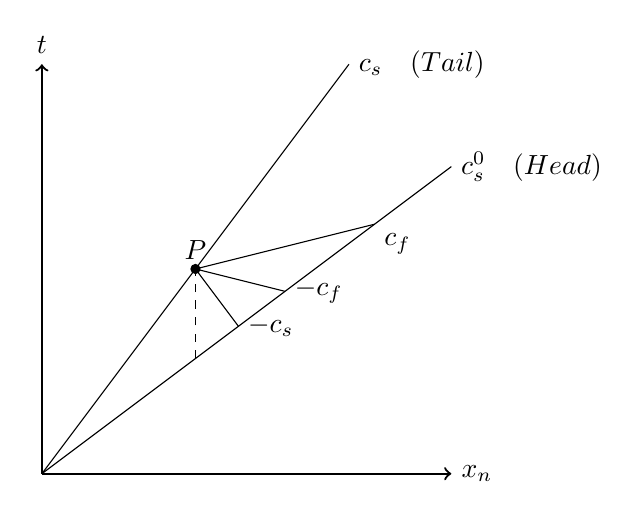
\begin{tikzpicture}[scale=1.3] 
  \newcommand\shift{5.}
  %% Slow
  \draw[thick,->] (0,0) -- (4.,0) node[right] {$x_n$};
  \draw[thick,->] (0,0) -- (0.,4) node[above] {$t$};
  % Slope = 0.75
  \draw (0,0) -- (4,3.) node [right] {$c_s^0 \quad (Head)$};
  % Slope = 4./3.
  \draw (0,0) -- (3.,4.) node [right] {$c_s \quad (Tail)$};

  \fill[black] (1.5,1.5*4./3.) circle (0.05) node [above] {$P$};
  %% Other characteristics
  % stationary
  \draw[dashed] (1.5,0.75*1.5) -- (1.5,1.5*4./3.);
  % fast plus (slope =+-0.25)
  \newcommand\px{1.5}
  \newcommand\py{1.5*4./3.}
  \draw (2.*\py-0.5*\px,1.5*\py-3.*\px/8.) node [below right] {$c_f$}-- (1.5,1.5*4./3.) ;
  % fast minus
  \draw (\py+0.25*\px,0.75*\py+3.*\px/16.) node [right] {$-c_f$} -- (1.5,1.5*4./3.) ;
  % slow minus (slope=-4./3.)
  \draw (12.*\py/25.+16.*\px/25.,9.*\py/25.+36.*\px/75.) node [right] {$-c_s$} -- (1.5,1.5*4./3.) ;
\end{tikzpicture}


%%% Local Variables:
%%% mode: latex
%%% TeX-master: "../../mainManuscript"
%%% End:
} \qquad
  \subcaptionbox{Fast simple wave \label{subfig:fastWave}}{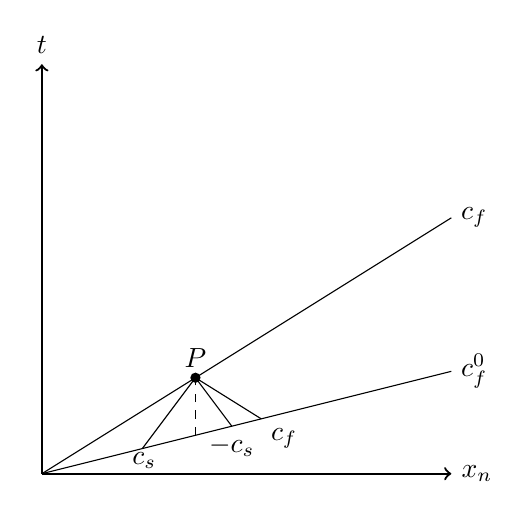
\begin{tikzpicture}[scale=1.3] 
  \newcommand\shift{5.}
  %% Fast
  \draw[thick,->] (0+\shift,0) -- (4.+\shift,0) node[right] {$x_n$};
  \draw[thick,->] (0+\shift,0) -- (0.+\shift,4) node[above] {$t$};
  % Slope = 0.25
  \draw (0+\shift,0) -- (4+\shift,1.) node [right] {$c_f^0$};
  % Slope = 5./8.
  \draw (0+\shift,0) -- (4+\shift,2.5) node [right] {$c_f$};
  
  \fill[black] (1.5+\shift,1.5*5./8.) circle (0.05) node [above] {$P$};
  %% Other characteristics
  \newcommand\pxx{1.5}
  \newcommand\pyy{1.5*5./8.}
  % stationary
  \draw[dashed] (1.5+\shift,1.5/4.) -- (\pxx+\shift,\pyy);
  % fast minus
  \draw (8.*\pyy/7.+5.*\pxx/7.+\shift,2.*\pyy/7.+10.*\pxx/56.) node [below right] {$c_f$}-- (\pxx+\shift,\pyy);
  % slow plus
  \draw (-12.0*\pyy/13.+16.*\pxx/13.+\shift,-3.*\pyy/13.+4.*\pxx/13.) -- (\pxx+\shift,\pyy);
  \node at (-12.0*\pyy/13.+16.*\pxx/13.+\shift+0.02,-3.*\pyy/13.+4.*\pxx/13.-0.12) {$c_s$};
  % slow minus
  \draw (12.0*\pyy/19.+16.*\pxx/19.+\shift,3.*\pyy/19.+4.*\pxx/19.)node [below] {$-c_s$} -- (\pxx+\shift,\pyy);
\end{tikzpicture}


%%% Local Variables:
%%% mode: latex
%%% TeX-master: "../../mainManuscript"
%%% End:
}
  \caption{The method of characteristics through slow and fast simple waves in the $(x_n,t)$ plane.}
  \label{fig:charac_method}
\end{figure}
The approach consists in tracing every characteristic from some downstream point of a wave where the state vector $\Qcb$ is known, to an upstream point where the solution is sought.
Figures \ref{fig:charac_method}\subref{subfig:slowWave} and \ref{fig:charac_method}\subref{subfig:fastWave} schematically illustrate the method for slow and fast simple waves in which the state is known along the head wave and is looked for at point $P$ lying on the tail wave. 
The integral curves through slow and fast simple waves are derived in the next section.

\subsection{Integral curves through simple waves}
The right-going slow waves are first looked at by adding equations \eqref{eq:charac_fr} and \eqref{eq:charac_fl}:
\begin{equation}
  l_i^1 n_j d\sigma_{ij}=0
\end{equation}
Given the geometry of the problem, the vector $\vect{n}$ may be reduced to $\vect{e}_1$ or $\vect{e}_2$.
It therefore comes out:
%In particular, for a vector $\vect{n}$ that is restricted to the axis of the $(\vect{e}_1,\vect{e}_2)$ plane, one gets:
\begin{subequations}
  \begin{alignat}{2}
    \label{eq:sigSlow_n=e1}
    & d\sigma_{11} = - \frac{l^1_2}{l_1^1} d\sigma_{12} = \psi^s_{1}d\sigma_{12} && \qquad \text{for } \:\vect{n}=\vect{e}_1 \\
    \label{eq:sigSlow_n=e2}
    & d\sigma_{22}=- \frac{l_1^1}{l_2^1}  d\sigma_{12} = \psi^s_{2}d\sigma_{12} && \qquad \text{for } \:\vect{n}=\vect{e}_2
  \end{alignat}
\end{subequations}
where $\psi^s_1$ and $\psi^s_2$ are functions of all components of $\tens{\sigma}$. 
Moreover, the $s$ and $f$ superscripts stand for slow and fast waves respectively in the remainder of the manuscript.
With the above equations, the characteristic equation related to the contact wave \eqref{eq:charac_contact} reads:
%Next, the characteristic equation related to the contact wave \eqref{eq:charac_contact} yields:
\begin{subequations}
  \begin{alignat}{2}
    \label{eq:sigContact_n=e1}
    & d\sigma_{22} = -\frac{\psi^s_{1}\alpha_{11}+\alpha_{12}}{\alpha_{22}}d\sigma_{12} && \qquad \text{for } \:\vect{n}=\vect{e}_1 \\
    \label{eq:sigContact_n=e2}
    & d\sigma_{11}= -\frac{\psi^s_{2}\alpha_{22}+\alpha_{12}}{\alpha_{11}} d\sigma_{12} && \qquad \text{for } \:\vect{n}=\vect{e}_2
  \end{alignat}
\end{subequations}
The sets of equations \eqref{eq:sigSlow_n=e1}-\eqref{eq:sigContact_n=e1} and \eqref{eq:sigSlow_n=e2}-\eqref{eq:sigContact_n=e2} show the combined-stress nature of slow simple waves.
% Hence, one stress component may be used as a driving parameter for the two others, as it is the case for $\sigma_{12}$ in equations \eqref{eq:sigSlow_n=e1}, \eqref{eq:sigSlow_n=e2}, \eqref{eq:sigContact_n=e1} and \eqref{eq:sigContact_n=e2}.
On the other hand, the subtraction of equations \eqref{eq:charac_fr} and \eqref{eq:charac_fl} leads to:
\begin{equation*}
  dv_1 = \psi^s_{1}dv_2 = \frac{1}{\psi^s_2}dv_2
\end{equation*}
which, once combined with equations \eqref{eq:sigSlow_n=e1}-\eqref{eq:sigSlow_n=e2} and introduced in \eqref{eq:charac_sl}, yields after simplifications:
\begin{subequations}
  \begin{alignat}{2}
    \label{eq:vSlow_n=e1}
    & dv_1 = -\frac{d\sigma_{11}}{\rho c_s^2} \quad ;\quad  dv_2 = -\frac{d\sigma_{12}}{\rho c_s^2} \qquad & \text{for } \vect{n}=\vect{e}_1\\
    \label{eq:vSlow_n=e2}
    & dv_1 = -\frac{d\sigma_{12}}{\rho c_s^2} \quad ;\quad  dv_2 = -\frac{d\sigma_{22}}{\rho c_s^2} \qquad & \text{for } \vect{n}=\vect{e}_2
  \end{alignat}
\end{subequations}

\begin{remark}
  The integral curves through a left-going slow wave result from the combination of equations \eqref{eq:sigSlow_n=e1}-\eqref{eq:sigSlow_n=e2} introduced in \eqref{eq:charac_sr} rather than \eqref{eq:charac_sl}.
  Therefore, the only difference lies in the signs in equations \eqref{eq:vSlow_n=e1} and \eqref{eq:vSlow_n=e2}.
\end{remark}

Similar results are obtained for right-going fast simple waves by using $\vect{l}^2$ instead of $\vect{l}^1$ and $c_f$ rather than $c_s$.
%However, the integral curves involve $\vect{l}^2$ and $c_f$ instead of $\vect{l}^1$ and $c_s$. 
Hence, the evolution in slow and fast waves is governed by the \textit{loading functions}:
\begin{equation}
  \label{eq:loading_func}
  \psi^s_{1}=- \left.\frac{l^1_2}{l_1^1}\right\rvert_{\vect{n}=\vect{e}_1}\quad ,\quad  \psi^s_{2}=- \left.\frac{l_1^1}{l_2^1}\right\rvert_{\vect{n}=\vect{e}_2} \quad ,\quad \psi^f_1=-\left.\frac{l_2^2}{l_1^2}\right\rvert_{\vect{n}=\vect{e}_1} \quad ,\quad \psi^f_2=-\left.\frac{l_1^2}{l_2^2}\right\rvert_{\vect{n}=\vect{e}_2}
\end{equation}
The equations satisfied across right-going slow and fast simple waves are summarized in table \ref{tab:simpleWavesEquations}.
\begin{table*}[h!]
  \centering
  \begin{tabular}{cc|ccN}
    \hline
    \multicolumn{2}{c}{Right-going slow wave} \vline& \multicolumn{2}{c}{Right-going fast wave} & \\
    $\vect{n}=\vect{e}_1$ & $\vect{n}=\vect{e}_2$ & $\vect{n}=\vect{e}_1$ & $\vect{n}=\vect{e}_2$&\\
    \hline
    \hline
    $dv_1 = -\frac{d\sigma_{11}}{\rho c_s^2}$ &  $dv_1 = -\frac{d\sigma_{12}}{\rho c_s^2}$ &$dv_1 = -\frac{d\sigma_{11}}{\rho c_f^2}$ &  $dv_1 = -\frac{d\sigma_{12}}{\rho c_f^2}$ &\\ [8pt]
    $dv_2 = -\frac{d\sigma_{12}}{\rho c_s^2}$ & $dv_2 = -\frac{d\sigma_{22}}{\rho c_s^2}$ & $dv_2 = -\frac{d\sigma_{12}}{\rho c_f^2}$ & $dv_2 = -\frac{d\sigma_{22}}{\rho c_f^2}$& \\ [8pt]
    $d\sigma_{11} = \psi^s_{1}d\sigma_{12}$&$d\sigma_{11}= -\frac{\psi^s_{2}\alpha_{22}+\alpha_{12}}{\alpha_{11}} d\sigma_{12}$ &  $d\sigma_{11} = \psi^f_{1}d\sigma_{12}$&$d\sigma_{11}= -\frac{\psi^f_{2}\alpha_{22}+\alpha_{12}}{\alpha_{11}} d\sigma_{12}$ & \\[8pt]
    $d\sigma_{22} = -\frac{\psi^s_{1}\alpha_{11}+\alpha_{12}}{\alpha_{22}}d\sigma_{12}$ & $d\sigma_{22}= \psi^s_{2}d\sigma_{12}$ & $d\sigma_{22} = -\frac{\psi^f_{1}\alpha_{11}+\alpha_{12}}{\alpha_{22}}d\sigma_{12}$ & $d\sigma_{22}= \psi^f_{2}d\sigma_{12}$ & \\[8pt]
    % & & \\
    % & & \\    
    \hline
\end{tabular}
%%% Local Variables:
%%% mode: latex
%%% TeX-master: "../manuscript"
%%% End:

  \caption{Summary of the ODEs satisfied inside right-going slow and fast simple waves.}
  \label{tab:simpleWavesEquations}
\end{table*}

The integration of equations gathered in table \ref{tab:simpleWavesEquations} should provide the complete solution of a given problem by means of integral curves, or loading paths.
For instance, the velocity resulting from the passage of right-going waves in the direction $\vect{e}_1$ obeys:
\begin{equation}
  \label{eq:integral_example}
  v_1 = v_1^0 - \int_{\tens{\sigma}^0}^{\tens{\sigma}} \frac{d \sigma_{11}}{\rho c^2} \quad ;\quad v_2 = v_2^0 - \int_{\tens{\sigma}^0}^{\tens{\sigma}} \frac{d \sigma_{12}}{\rho c^2}
\end{equation}
where the zero superscript denotes the downstream state.
Nevertheless, \textsc{Clifton} \cite{Clifton} emphasized that depending on the loading conditions, only one simple wave or both may arise in the solution.
Therefore, it is crucial to identify the stress path followed to properly compute integrals \eqref{eq:integral_example}.
%It is thus important to qualify the stress paths through fast and slow waves in order to properly define the upper bound of the integrals of the form \eqref{eq:integral_example}.
This is the purpose of the next section.

%%% Local Variables:
%%% mode: latex
%%% TeX-master: "manuscript"
%%% End:
